\begin{usecase}{Schedule Prayer Times}
  \ucbasicinfo{High}{Regular}
  \ucshortdescription{The calendar is blocked and updated automatically according to the person's time zone prayer time.}
  \uctrigger{This usecase triggered when the user enables the prayer time feature in the application.}
  \ucactors{User}{None}
  \ucpreconditions{User must be logged into the system.}
  \ucrelationships{N/A}{N/A}{N/A}
  \ucinputsoutputs{
    \begin{itemize}
      \item \textbf{User's time Zone} (Source: user)
      \item \textbf{We get the IP address of the user and get their time zone}
    \end{itemize}
  }{
    \begin{itemize}
      \item \textbf{The calendar displays the blocked time for prayer time according to their time zone.}
    \end{itemize}
  }
  \ucmainflow{
    \begin{enumerate}
      \item User enables the feature by clicking the the option Schedule Prayer Time.
            \ucinfo{The system checks the time zone of the user and blocks the calendar accordingly.}
    \end{enumerate}
  }
  \ucalternateflows{
    \begin{itemize}
      \item The user doesn't enable the scheduling prayer time.
    \end{itemize}
  }
  \ucexceptions{
    \begin{itemize}
      \item If there's a system error, display a relevant error message.
    \end{itemize}
  }
  \ucpostconditions{The system generates calendar with prayer time}
  \ucspecialrequirements{The system must block the calendar according to their time zone}
  \ucconclusion{User's prayer times are successfully scheduled.}
  \ucbusinessrules{
    \begin{itemize}
      \item Prayer times must be within valid time ranges.
    \end{itemize}
  }
\end{usecase}

\begin{figure}[!h]
  \centering
  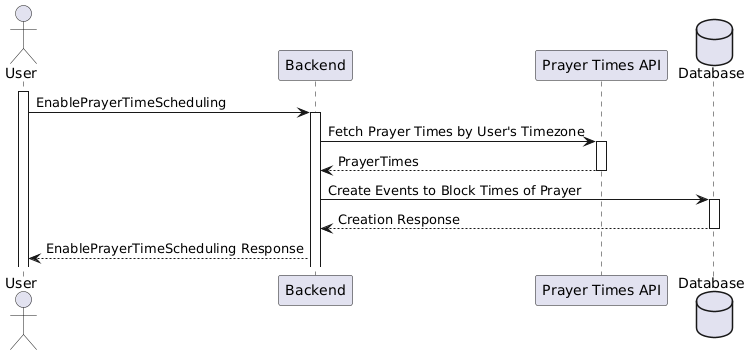
\includegraphics[width=\textwidth]{images/docs/diagrams/sequence-diagrams/all-sequence-diagrams/Schedule Prayer Times.png}
  \caption{Schedule Prayer Times Sequence Diagram}
  \label{fig:seq/schedule-prayer-times}
\end{figure}

The "Schedule Prayer Times Sequence Diagram", shown in \textbf{Figure~\ref{fig:seq/schedule-prayer-times}}, illustrates Jadwal's unique feature of automatically scheduling prayer times based on the user's timezone. The process begins when the user initiates the EnablePrayerTimeScheduling gRPC call to activate this feature.

Upon activation, the sequence follows these steps:
\begin{enumerate}
  \item The Backend determines the user's timezone and queries the Prayer Times API for accurate prayer schedules
  \item The Prayer Times API returns the specific times for each prayer based on the user's location
  \item The Backend creates blocking events in the Database for each prayer time
  \item A confirmation response is sent back to the user through the gRPC channel
\end{enumerate}

This automated process ensures that:
\begin{itemize}
  \item Prayer times are accurately calculated based on geographical location
  \item Calendar blocking is automatically adjusted for timezone changes
  \item Users can maintain their prayer schedule while managing other commitments
\end{itemize}

The system's ability to automatically block out prayer times demonstrates Jadwal's commitment to supporting users' religious obligations while maintaining efficient schedule management.